\section{Computer networks}
\begin{itemize}
    \item A computer network is a system in which multiple computers are connected to each other to share information and resources.
    \item Characteristics of a computer network:
        \begin{itemize}
            \item Share resources from one computer to another.
            \item Create files and store them in one computer, access those files from the other computers connected over the network.
            \item Connect a printer, scanner, or a fax machine to one computer within the network and let other computers of the network use the machines available over the network.
        \end{itemize}
    
    \item Hardware required to setup the computer network:
        \begin{itemize}
            \item Network cables: ethernet cables.
                \begin{itemize}
                    \item 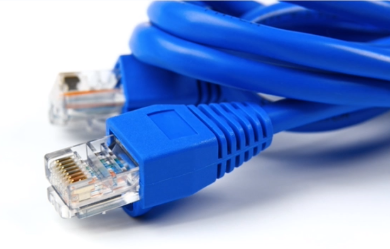
\includegraphics[width=\width\textwidth]{./figs/20230208192012.png}
                \end{itemize}
            
            \item Distributors:
                \begin{figure}[H]
                    \centering
                    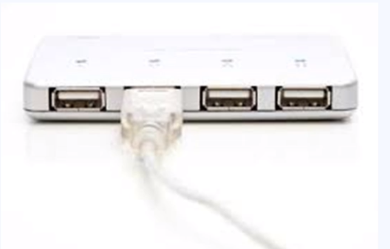
\includegraphics[width=\width\textwidth]{./figs/20230208192032.png}
                    %\caption{}
                \end{figure}
            
            \item Router:
                \begin{figure}[H]
                    \centering
                    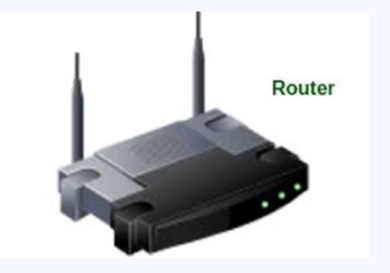
\includegraphics[width=\width\textwidth]{./figs/20230208192055.png}
                    %\caption{}
                \end{figure}
            
            \item Network card:
                \begin{figure}[H]
                    \centering
                    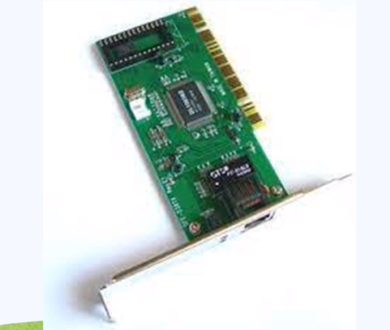
\includegraphics[width=\width\textwidth]{./figs/20230208192113.png}
                    %\caption{}
                \end{figure}
            
            \item Universal Serial Bus: USB:
                \begin{figure}[H]
                    \centering
                    
\includegraphics[width=\width\textwidth]{./figs/20230208192139.png}
                    %\caption{}
                \end{figure}
        \end{itemize}
    
    \item Types of computer networks:
        \begin{itemize}
            \item There are basically 4 types: PAN, LAN, MAN, WAN.
                \begin{itemize}
                    \item PAN: Personal Area Network.
                    \item LAN: Local Area Network.
                    \item MAN: Metropolitan Area Network.
                    \item WAN: Wide Area Network.
                \end{itemize}
            
            \item LAN: stands for Local Area Network: it is a computer network that has 2 or more connected computers, and is contained within a small geographic area, usually within the same building. Home WiFi networks and small business networks are common examples.
                \begin{figure}[H]
                    \centering
                    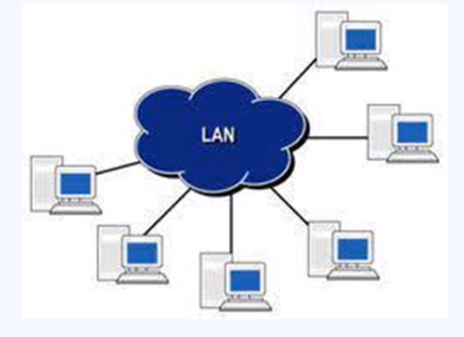
\includegraphics[width=\width\textwidth]{./figs/20230208192500.png}
                    %\caption{}
                \end{figure}

            \item PAN: Personal Area Network: is a computer network that connects computers and devices within the range of an individual person. A PAN provides a network range within a person's range typically within a range of 10 meters or 33 feet. 
                \begin{figure}[H]
                    \centering
                    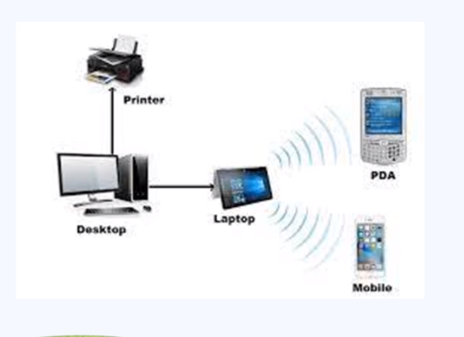
\includegraphics[width=\width\textwidth]{./figs/20230208192647.png}
                    %\caption{}
                \end{figure}
            
            \item MAN: A metropolitan area network is a network in which private data is exchanged, usually used by a single organization in several buildings that are all interconnected in the same geographic vicinity. It is larger than a LAN in a single building but not large enough to be considered a WAN. The size usually ranges from 5 kilometers to 50 kilometers. If all the buildings are in the same piece of contigous property, it may also be considered a campus network.
                \begin{figure}[H]
                    \centering
                    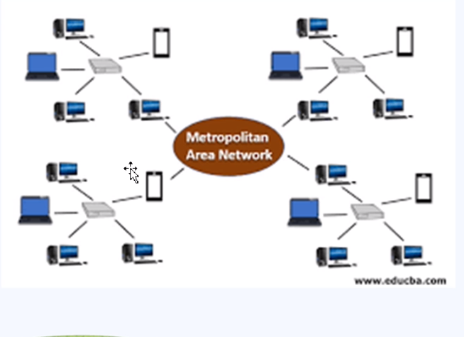
\includegraphics[width=\width\textwidth]{./figs/20230208231829.png}
                    %\caption{}
                \end{figure}
            
            \item WAN: Wide Area Network: is a greographical area consisting of 2 or more LANs or MANs. These networks are established with leased telecommunication circuits, in which two sides which are connected have routers that connect the LAN of both sides together in a network to facilitate communication.
                \begin{figure}[H]
                    \centering
                    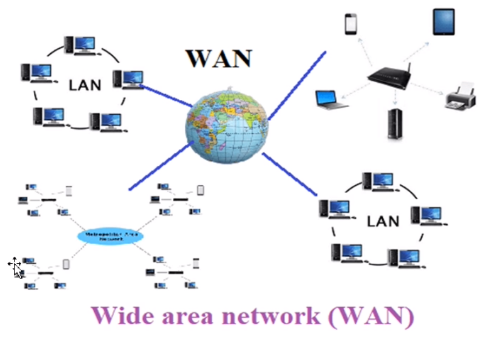
\includegraphics[width=\width\textwidth]{./figs/20230208232028.png}
                    %\caption{}
                \end{figure}
        \end{itemize}
\end{itemize}

%%%%%%%%%%%%%%%%%%%%%%%%%%%%%%%%%%%%%%%%%%%%%%%%%%%%%%
\section{Topology and it's types}
\begin{itemize}
    \item A topology: is derived from two greek words, topo and logy. Where topo means place and logy means study. In computer networks, a topology is used to explain how a network is physically connected and the logical flow of information in the network.
    \item There are 2 types of topology.
        \begin{enumerate}
            \item Physical topology.
            \item Logical topology.
        \end{enumerate}
    
    \item Now to explain the physical topology:
        \begin{itemize}
            \item A physical topology describes the way in which the computers or nodes are connected with each other in a computer network. It is the arrangement of various elements (link, nodes, etc.) including the device location and code installation of a computer network. In other words... we can say that it is the phycial layout of nodes, workstations, and cables in the network.
        \end{itemize}
    
    \item Logical topology:
        \begin{itemize}
            \item A logical topology describes the way, data flow from one computer to anoter. 
            \item It is bound to a network protocol and defines how data is moved throughout the network and which path it takes. 
            \item In other words, it is the way in which the devices communicate internally.
        \end{itemize}
    
    \item In a computer network, there are mainly six types of topology.
        \begin{enumerate}
            \item Bus topology.
            \item Ring topology.
            \item Star topology.
            \item Mesh topology.
            \item Tree topology.
            \item Hybrid topology.
        \end{enumerate}
    
    \item Bus topology: A bus topology is the simplest kind of topology in which a common bus or channel is used for communication in the network. The bus is connected to various taps and droplines.
        \begin{figure}[H]
            \centering
            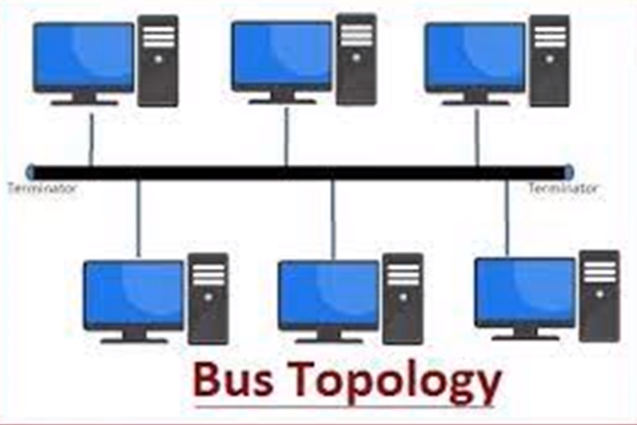
\includegraphics[width=\width\textwidth]{./figs/20230208233514.png}
            %\caption{}
        \end{figure}
        \begin{itemize}
            \item It has certain advantages: for example it is simpler to set up and if one node fails it will not affect other nodes.
        \end{itemize}
    
    \item Ring topology: in this one the computer is connected to exactly two other computers to form the ring. The message passing is unidirectional.
        \begin{figure}[H]
            \centering
            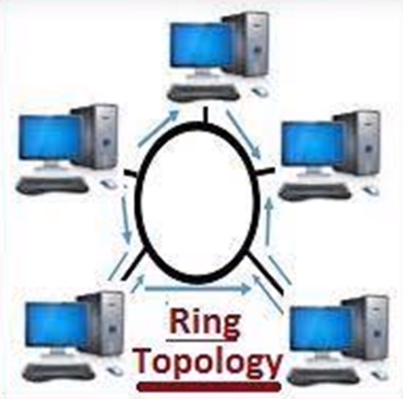
\includegraphics[width=\width\textwidth]{./figs/20230208233710.png}
            %\caption{}
        \end{figure}
        \begin{itemize}
            \item The one disadvantage is that if one node fails the whole network fails.
        \end{itemize}
    
    \item Star topology: is a computer network in which all the nodes are connected to a centralized hub.
        \begin{figure}[H]
            \centering
            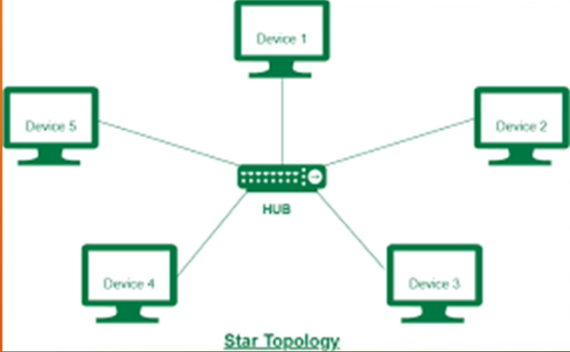
\includegraphics[width=\width\textwidth]{./figs/20230208233854.png}
            %\caption{}
        \end{figure}
        \begin{itemize}
            \item This topology is better in terms of security.
            \item The data does not pass through every node. 
            \item Easy to troubleshoot and easy to scale.
        \end{itemize}
    
    \item Mesh topology: is a computer network topology in which nodes are interconnected with each other.
        \begin{figure}[H]
            \centering
            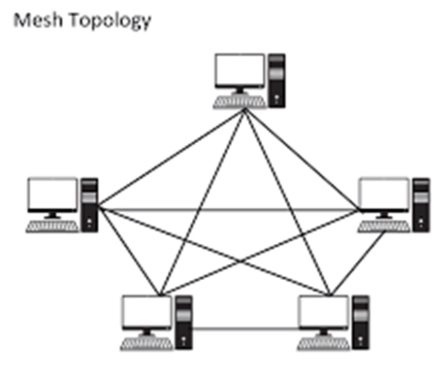
\includegraphics[width=\width\textwidth]{./figs/20230208233959.png}
            %\caption{}
        \end{figure}
        \begin{itemize}
            \item In this topology there is a more direct line of communication. Much faster.
            \item If one node fails the network still works.
        \end{itemize}
    
    \item Tree topology: is a computer network topology in which all the nodes are directly or indirectly connected to the main bus cable.
        \begin{figure}[H]
            \centering
            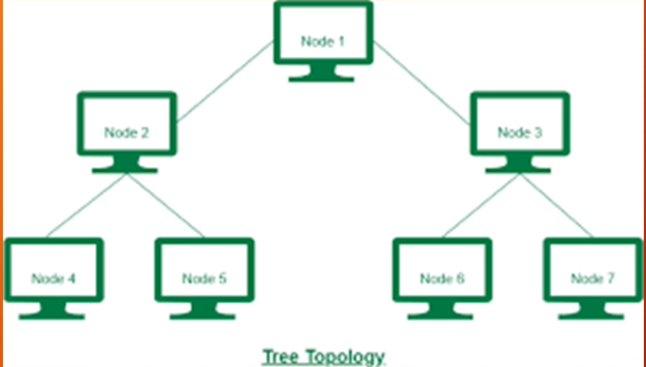
\includegraphics[width=\width\textwidth]{./figs/20230208234147.png}
            %\caption{}
        \end{figure}
        \begin{itemize}
            \item It is a combination of a bus and star topology.
        \end{itemize}
    
    \item Hybrid topology: topology in which there is a combination of two or more topologies.
        \begin{figure}[H]
            \centering
            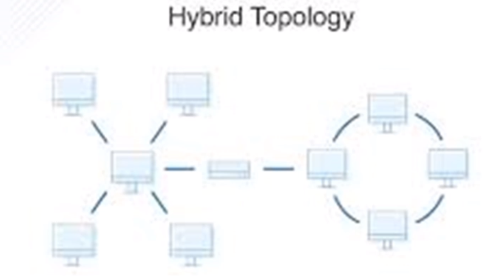
\includegraphics[width=\width\textwidth]{./figs/20230208234314.png}
            %\caption{}
        \end{figure}
        \begin{itemize}
            \item These are the more used in the real world.
            \item Can handle a large number of nodes.
            \item Provides flexibility to modify the network according to our needs.
        \end{itemize}
\end{itemize}